\section{Použití - medicína}

\begin{frame}
	\frametitle{Důležité vlastnosti}
	\begin{itemize}
		\item Nezpůsobuje alergické reakce
		\item V těle neprobíhají chemické reakce s tímto materiálem
		\item Nezpůsobuje záněty či šíření infekcí
		\item Bezpečné a pohodlné použití
	\end{itemize}
\end{frame}

\begin{frame}
	\frametitle{Cévní náhrady}
	\begin{itemize}
		\item Silný materiál
		\item Možnost pružné varianty
	\end{itemize}
	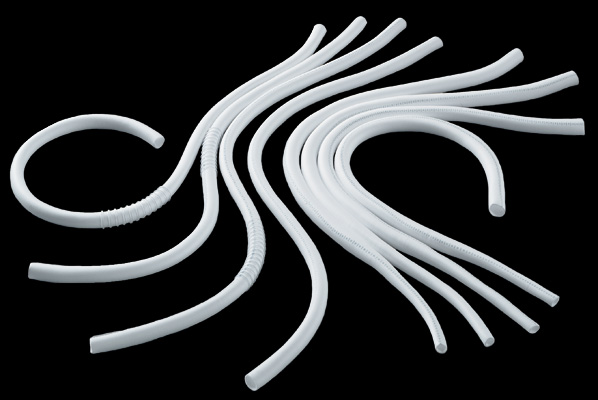
\includegraphics[width=0.6\textwidth]{nahradni_ceva.jpg}
	\zdroj{http://www.goremedical.com/resources/images/popups/vgstretch.jpg}
\end{frame}

\begin{frame}
	\frametitle{Stehy}
	\begin{columns}
	\begin{column}{0.5\textwidth}
	\begin{itemize}
		\item Jemné, ohebné a pružné vlákno
		\item Nemá paměťový efekt
		\item Jehla stejně velká jako vlákno - zabraňuje úniku dírou po jehle 
	\end{itemize}
	\end{column}
	\begin{column}{0.5\textwidth}
		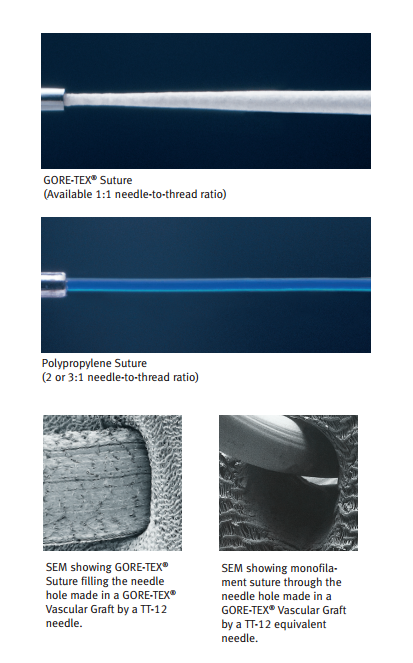
\includegraphics[scale=0.38]{needle_thread.png}
	\end{column}
	\end{columns}
	\zdroj{http://www.goremedical.com/resources/dam/assets/AB0101-EN6.pdf}
\end{frame}

\begin{frame}
	\frametitle{Další použití v medicíně}
	\begin{itemize}
		\item Operace trávicího traktu
		\item Operace srdce a plic
		\item Náhrada uložení páteřních cév
		\item Operace kýly
		\item Obecná chirurgie - záplaty, vlákna, ochrany
	\end{itemize}
\end{frame}